% Dynamic Programming Part 1 -- Metropolis beamer slides
% Compile: pdflatex dynamic-programming-1.tex (x2)
\documentclass[10pt,aspectratio=169]{beamer}

\usetheme{metropolis}
\metroset{block=fill, numbering=fraction, progressbar=frametitle}

\usepackage[T1]{fontenc}
\usepackage{amsmath, amssymb}
\usepackage{listings}
\usepackage{booktabs}
\usepackage{tikz}
\usepackage{pgfplots}
\pgfplotsset{compat=1.18}
\usetikzlibrary{arrows.meta, positioning, decorations.pathreplacing, calc, matrix}

% ---- colors -------------------------------------------------------------
\definecolor{mLightBlue}{HTML}{4C72B0}
\definecolor{mGreen}{HTML}{55A868}
\definecolor{mRed}{HTML}{C44E52}
\definecolor{mGray}{HTML}{BFBFBF}
\setbeamercolor{alerted text}{fg=mRed}

% ---- code style ---------------------------------------------------------
\lstdefinestyle{jl}{
  basicstyle=\ttfamily\footnotesize,
  keywordstyle=\color{mRed}\bfseries,
  commentstyle=\color{mGreen}\itshape,
  numberstyle=\tiny\color{mGray},
  showstringspaces=false,
  breaklines=true,
  columns=fullflexible,
  morekeywords={function,for,in,if,else,elseif,end,return,length,while,using}
}
\lstset{style=jl}

% ---- helpers ------------------------------------------------------------
% one row of an alignment table: \alignrow{y}{list of letters}{list of fills}
\newcommand{\alignrow}[3]{%
  \foreach \v/\fillc [count=\i from 0] in {#2} {
    \node[draw, minimum size=7mm, fill=\fillc] at (\i*0.8,#1) {\small \tt \v};
  }%
}

% ---- title --------------------------------------------------------------
\title{Dynamic Programming, Part 1}
\subtitle{Fibonacci, Shortest Path in DAGs, LIS, Edit Distance}
\date{}
\author{}

\begin{document}

\maketitle

% =========================================================================
\begin{frame}{Dynamic Programming}
  \begin{center}
    \Large
    Recursion \; $+$ \; memoization.
  \end{center}

  % \bigskip
  % \pause

  % Three questions to ask every time:

  % \begin{itemize}
  %   \item What is the \alert{table}?
  %   \item What are the \alert{base cases}?
  %   \item How do we \alert{fill} the dynamic  ptable?
  % \end{itemize}
\end{frame}

% =========================================================================
\section{Fibonacci}

\begin{frame}{The Sequence}
  $F_0 = 0$, \; $F_1 = 1$, \; and $F_i = F_{i-1} + F_{i-2}$ for $i > 1$.

  \bigskip
  \begin{center}
  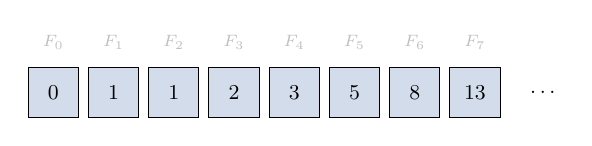
\begin{tikzpicture}[scale=0.85, every node/.style={transform shape}]
    \foreach \v [count=\i from 0] in {0,1,1,2,3,5,8,13} {
      \node[draw, minimum size=7.5mm, fill=mLightBlue!25] at (\i*0.9,0) {\small \v};
      \node[mGray] at (\i*0.9,0.75) {\scriptsize $F_{\i}$};
    }
    \node[right] at (7.0,0) {\small $\ldots$};
  \end{tikzpicture}
  \end{center}

  \bigskip
  The definition is recursive, so the obvious algorithm is too.
\end{frame}

\begin{frame}[fragile]{The Obvious Algorithm}
  \begin{lstlisting}
function fibonacci(i)
    if i == 0
        return 0
    elseif i == 1
        return 1
    else
        return fibonacci(i - 1) + fibonacci(i - 2)
    end
end
  \end{lstlisting}

  \bigskip
  Its running time satisfies
  \[
    T(n) = T(n-1) + T(n-2) + O(1) \;\ge\; 2\,T(n-2) + c.
  \]
\end{frame}

\begin{frame}{Exercise}
  \begin{center}
    Use the recursion tree method to show that \texttt{fibonacci} takes
    exponential time.
  \end{center}

  \bigskip
  \begin{center}
    \small Start from $T(n) \ge 2\,T(n-2) + c$.
  \end{center}
\end{frame}

\begin{frame}{Solution}
  Unroll the inequality. Each level \alert{doubles} the number of calls while
  the argument drops by $2$:
  \[
    T(n) \;\ge\; 2\,T(n-2) \;\ge\; 4\,T(n-4) \;\ge\; \cdots \;\ge\; 2^k\,T(n-2k).
  \]

  \bigskip
  The base case is reached at $k = n/2$, so
  \[
    T(n) \;\ge\; 2^{n/2} = \left(\sqrt{2}\right)^{n}.
  \]

  \bigskip
  \begin{center}
    \small The exact growth is $\Theta(\varphi^n)$ with
    $\varphi = \frac{1+\sqrt5}{2} \approx 1.618$, but any exponential lower
    bound makes the point.
  \end{center}
\end{frame}

\begin{frame}{Why It Is Wasteful}
  \begin{center}
  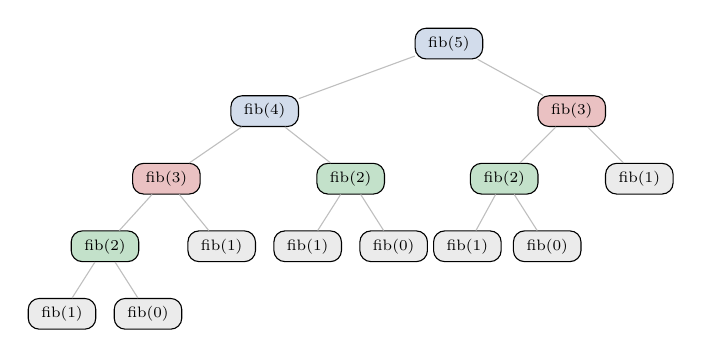
\begin{tikzpicture}[scale=0.78, every node/.style={transform shape},
      nd/.style={draw, rounded corners, minimum width=11mm, minimum height=5mm,
                 inner sep=1pt, font=\scriptsize}]
    \node[nd, fill=mLightBlue!25] (f5) at (0,0) {fib(5)};
    \node[nd, fill=mLightBlue!25] (f4) at (-3.0,-1.1) {fib(4)};
    \node[nd, fill=mRed!35]       (f3a) at (2.0,-1.1) {fib(3)};
    \node[nd, fill=mRed!35]       (f3b) at (-4.6,-2.2) {fib(3)};
    \node[nd, fill=mGreen!35]     (f2a) at (-1.6,-2.2) {fib(2)};
    \node[nd, fill=mGreen!35]     (f2b) at (0.9,-2.2) {fib(2)};
    \node[nd, fill=black!8]       (f1a) at (3.1,-2.2) {fib(1)};
    \node[nd, fill=mGreen!35]     (f2c) at (-5.6,-3.3) {fib(2)};
    \node[nd, fill=black!8]       (f1b) at (-3.7,-3.3) {fib(1)};
    \node[nd, fill=black!8]       (f1c) at (-2.3,-3.3) {fib(1)};
    \node[nd, fill=black!8]       (f0a) at (-0.9,-3.3) {fib(0)};
    \node[nd, fill=black!8]       (f1d) at (0.3,-3.3) {fib(1)};
    \node[nd, fill=black!8]       (f0b) at (1.6,-3.3) {fib(0)};
    \node[nd, fill=black!8]       (f1e) at (-6.3,-4.4) {fib(1)};
    \node[nd, fill=black!8]       (f0c) at (-4.9,-4.4) {fib(0)};
    \foreach \a/\b in {f5/f4, f5/f3a, f4/f3b, f4/f2a, f3a/f2b, f3a/f1a,
                       f3b/f2c, f3b/f1b, f2a/f1c, f2a/f0a, f2b/f1d, f2b/f0b,
                       f2c/f1e, f2c/f0c}
      \draw[mGray] (\a) -- (\b);
  \end{tikzpicture}
  \end{center}

  \begin{center}
    \small \textcolor{mRed}{fib(3)} twice, \textcolor{mGreen}{fib(2)} three
    times, and it only gets worse.
  \end{center}
\end{frame}

\begin{frame}[fragile]{Top-Down: Memoization}
  Before recursing, check whether the answer is already known.

  \begin{lstlisting}[basicstyle=\ttfamily\scriptsize]
function compute_fibonacci(n)
    F = OffsetArray(fill(nothing, n + 1), 0:n)
    F[0] = 0
    F[1] = 1

    function fib(i)
        if i == 0 || i == 1
            return F[i]
        else
            if isnothing(F[i - 1]); fib(i - 1); end
            if isnothing(F[i - 2]); fib(i - 2); end
            F[i] = F[i - 1] + F[i - 2]
            return F[i]
        end
    end

    return fib(n)
end
  \end{lstlisting}
\end{frame}

\begin{frame}[fragile]{Bottom-Up}
  Or fill the table deliberately, left to right.

  \begin{lstlisting}
function fibonacci_bottom_up(n)
    F = OffsetArray(zeros(Int, n + 1), 0:n)
    F[0] = 0
    F[1] = 1
    for i in 2:n
        F[i] = F[i - 1] + F[i - 2]
    end
    return F[n]
end
  \end{lstlisting}

  \bigskip
  \begin{center}
  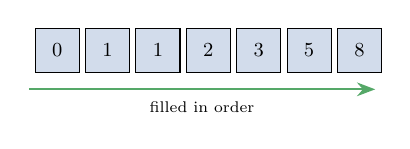
\begin{tikzpicture}[scale=0.8, every node/.style={transform shape}]
    \foreach \v [count=\i from 0] in {0,1,1,2,3,5,8} {
      \node[draw, minimum size=7mm, fill=mLightBlue!25] at (\i*0.8,0) {\small \v};
    }
    \draw[-{Stealth}, thick, mGreen] (-0.45,-0.62) -- (5.05,-0.62);
    \node[below] at (2.3,-0.7) {\scriptsize filled in order};
  \end{tikzpicture}
  \end{center}

  \begin{center}
    Exponential becomes $O(n)$.
  \end{center}
\end{frame}

% =========================================================================
\section{Shortest Path in DAGs}

\begin{frame}{Setup}
  Vertices $v_1, \ldots, v_n$ in \alert{topological order}: every edge goes
  from $v_i$ to $v_j$ with $i < j$.

  \bigskip
  \begin{itemize}
    \item $W[v_i, v_j]$ is the length of the edge $v_i \to v_j$.
    \item $\text{incoming}(v_i)$ lists the vertices with an edge into $v_i$.
  \end{itemize}

  \bigskip
  \begin{center}
    Such a graph has no cycle. Why?
  \end{center}

  \bigskip
  \begin{center}
    \small Goal: compute $dist[i]$, the shortest path length from $v_1$ to $v_i$.
  \end{center}
\end{frame}

\begin{frame}{An Example DAG}
  \begin{center}
  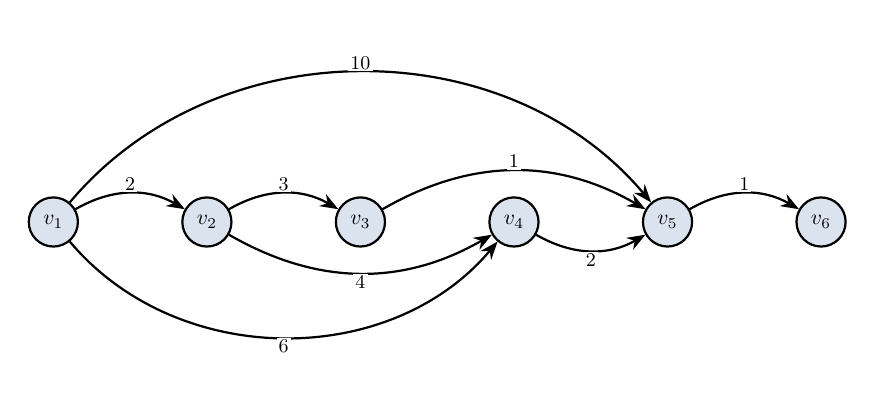
\begin{tikzpicture}[scale=0.78, every node/.style={transform shape},
      >=Stealth, thick,
      vtx/.style={circle, draw, minimum size=8mm, inner sep=1pt,
                  fill=mLightBlue!20},
      lbl/.style={draw=none, minimum size=0, fill=white, inner sep=1pt,
                  font=\small}]
    \node[vtx] (v1) at (0,0) {$v_1$};
    \node[vtx] (v2) at (2.5,0) {$v_2$};
    \node[vtx] (v3) at (5,0) {$v_3$};
    \node[vtx] (v4) at (7.5,0) {$v_4$};
    \node[vtx] (v5) at (10,0) {$v_5$};
    \node[vtx] (v6) at (12.5,0) {$v_6$};

    \draw[->] (v1) to[bend left=30]  node[lbl, above] {2}  (v2);
    \draw[->] (v2) to[bend left=30]  node[lbl, above] {3}  (v3);
    \draw[->] (v2) to[bend right=30] node[lbl, below] {4}  (v4);
    \draw[->] (v3) to[bend left=30]  node[lbl, above] {1}  (v5);
    \draw[->] (v4) to[bend right=30] node[lbl, below] {2}  (v5);
    \draw[->] (v5) to[bend left=30]  node[lbl, above] {1}  (v6);
    \draw[->] (v1) to[bend right=50] node[lbl, below] {6}  (v4);
    \draw[->] (v1) to[bend left=50]  node[lbl, above] {10} (v5);
  \end{tikzpicture}
  \end{center}

  \bigskip
  \begin{center}
    $\text{incoming}(v_5) = \{v_1, v_3, v_4\}$ with
    $W[v_1,v_5] = 10$, \; $W[v_3,v_5] = 1$, \; $W[v_4,v_5] = 2$.
  \end{center}
\end{frame}

\begin{frame}{The Recurrence}
  \begin{itemize}
    \item $dist[1] = 0$: the shortest path from $v_1$ to itself is just $v_1$.
    \pause
    \item Any path to $v_i$ arrives through some predecessor $v_j$, using the
          edge $v_j \to v_i$.
    \pause
    \item If it passes through $v_j$, its length is
          (shortest path to $v_j$) $+$ $W[v_j, v_i]$.
  \end{itemize}

  \pause
  \bigskip
  \begin{alertblock}{}
    \[
      dist[v_i] = \min_{j < i \,:\, v_j \to v_i \in E}
                  \Big( dist[v_j] + W[v_j, v_i] \Big)
    \]
  \end{alertblock}

  \bigskip
  \begin{center}
    Everything on the right is to the \alert{left} of $i$, so fill left to right.
  \end{center}
\end{frame}

\begin{frame}{Working the Example}
  \begin{center}
  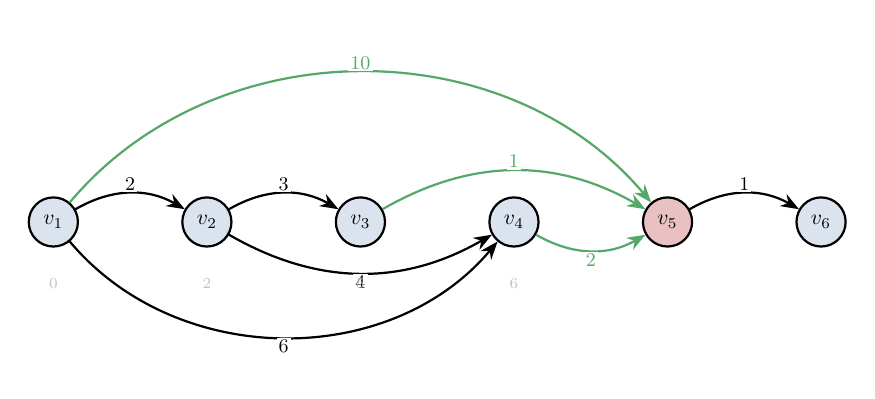
\begin{tikzpicture}[scale=0.78, every node/.style={transform shape},
      >=Stealth, thick,
      vtx/.style={circle, draw, minimum size=8mm, inner sep=1pt,
                  fill=mLightBlue!20},
      lbl/.style={draw=none, minimum size=0, fill=white, inner sep=1pt,
                  font=\small}]
    \node[vtx] (v1) at (0,0) {$v_1$};
    \node[vtx] (v2) at (2.5,0) {$v_2$};
    \node[vtx] (v3) at (5,0) {$v_3$};
    \node[vtx] (v4) at (7.5,0) {$v_4$};
    \node[vtx, fill=mRed!35] (v5) at (10,0) {$v_5$};
    \node[vtx] (v6) at (12.5,0) {$v_6$};

    \draw[->] (v1) to[bend left=30]  node[lbl, above] {2}  (v2);
    \draw[->] (v2) to[bend left=30]  node[lbl, above] {3}  (v3);
    \draw[->] (v2) to[bend right=30] node[lbl, below] {4}  (v4);
    \draw[->, mGreen] (v3) to[bend left=30]  node[lbl, above] {1}  (v5);
    \draw[->, mGreen] (v4) to[bend right=30] node[lbl, below] {2}  (v5);
    \draw[->] (v5) to[bend left=30]  node[lbl, above] {1}  (v6);
    \draw[->] (v1) to[bend right=50] node[lbl, below] {6}  (v4);
    \draw[->, mGreen] (v1) to[bend left=50]  node[lbl, above] {10} (v5);

    \node[mGray, draw=none, fill=none] at (0,-1.0)  {\scriptsize $0$};
    \node[mGray, draw=none, fill=none] at (2.5,-1.0) {\scriptsize $2$};
    \node[mGray, draw=none, fill=none] at (5,-1.0)   {\scriptsize $5$};
    \node[mGray, draw=none, fill=none] at (7.5,-1.0) {\scriptsize $6$};
  \end{tikzpicture}
  \end{center}

  \[
    dist[v_5] = \min\big(\underbrace{0 + 10}_{v_1},\;
                         \underbrace{5 + 1}_{v_3},\;
                         \underbrace{6 + 2}_{v_4}\big) = 6.
  \]
\end{frame}

\begin{frame}{Reconstructing the Path}
  If the shortest path to $v_i$ arrives from $v_j$, then the shortest path to
  $v_j$ is a \alert{prefix} of it.

  \bigskip
  So record a predecessor $\pi[i] = j$ each time we improve $dist[i]$, and walk
  backwards from the target.

  \bigskip
  \begin{center}
  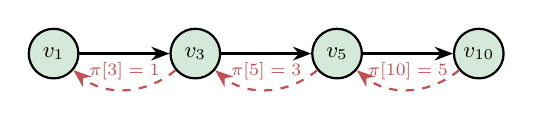
\begin{tikzpicture}[scale=0.9, every node/.style={transform shape},
      >=Stealth, thick,
      vtx/.style={circle, draw, minimum size=7mm, inner sep=1pt,
                  fill=mGreen!25, font=\small}]
    \node[vtx] (a) at (0,0)   {$v_1$};
    \node[vtx] (b) at (2,0)   {$v_3$};
    \node[vtx] (c) at (4,0)   {$v_5$};
    \node[vtx] (d) at (6,0)   {$v_{10}$};
    \draw[->] (a) -- (b); \draw[->] (b) -- (c); \draw[->] (c) -- (d);
    \draw[->, mRed, dashed] (d) to[bend left=40] node[above, draw=none, fill=none, font=\scriptsize] {$\pi[10]=5$} (c);
    \draw[->, mRed, dashed] (c) to[bend left=40] node[above, draw=none, fill=none, font=\scriptsize] {$\pi[5]=3$} (b);
    \draw[->, mRed, dashed] (b) to[bend left=40] node[above, draw=none, fill=none, font=\scriptsize] {$\pi[3]=1$} (a);
  \end{tikzpicture}
  \end{center}
\end{frame}

\begin{frame}[fragile]{Implementation}
  \begin{lstlisting}
function shortest_path_dag(n, incoming, W)
    dist = fill(Inf, n)
    p = fill(0, n)      # p[i] = predecessor of v_i
    dist[1] = 0

    for i in 2:n
        for vj in incoming[i]
            if dist[vj] + W[vj, i] < dist[i]
                dist[i] = dist[vj] + W[vj, i]
                p[i] = vj
            end
        end
    end

    return dist, p
end
  \end{lstlisting}
\end{frame}

\begin{frame}{Running Time}
  \begin{itemize}
    \item The outer loop runs $O(|V|)$ times.
    \item The inner loop walks the incoming edges of $v_i$.
    \item Across all $i$, each edge is examined \alert{exactly once}.
  \end{itemize}

  \bigskip
  \begin{alertblock}{}
    \[
      O(|V| + |E|)
    \]
  \end{alertblock}
\end{frame}

% =========================================================================
\section{Longest Increasing Subsequence}

\begin{frame}{The Problem}
  Given $A[1 \ldots n]$, find the longest increasing subsequence.

  \bigskip
  \begin{center}
  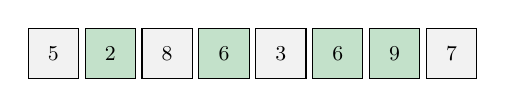
\begin{tikzpicture}[scale=0.85, every node/.style={transform shape}]
    \foreach \v/\fillc [count=\i from 0] in
      {5/black!5, 2/mGreen!35, 8/black!5, 6/mGreen!35, 3/black!5, 6/mGreen!35, 9/mGreen!35, 7/black!5} {
      \node[draw, minimum size=7.5mm, fill=\fillc] at (\i*0.85,0) {\small \v};
    }
  \end{tikzpicture}
  \end{center}

  \bigskip
  \begin{center}
    \small Highlighted: $2, 6, 6, 9$ of length $4$.
  \end{center}

  \bigskip
  \textbf{Motivation:} one way to measure how sorted a database is. If the LIS
  is close to $n$, the data is nearly sorted.
\end{frame}

\begin{frame}{Reduce It to a Longest Path}
  Build a graph: node $i$ for $A[i]$, and an edge $j \to i$ of length $1$
  whenever $j < i$ and $A[j] \le A[i]$.

  \bigskip
  \begin{center}
  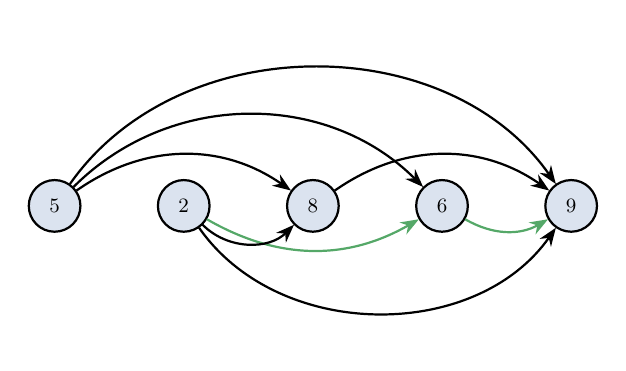
\begin{tikzpicture}[scale=0.82, every node/.style={transform shape},
      >=Stealth, thick,
      vtx/.style={circle, draw, minimum size=8mm, inner sep=1pt,
                  fill=mLightBlue!20, font=\small}]
    \node[vtx] (a) at (0,0)  {$5$};
    \node[vtx] (b) at (2,0)  {$2$};
    \node[vtx] (c) at (4,0)  {$8$};
    \node[vtx] (d) at (6,0)  {$6$};
    \node[vtx] (e) at (8,0)  {$9$};
    \draw[->] (a) to[bend left=35] (c);
    \draw[->] (a) to[bend left=45] (d);
    \draw[->] (a) to[bend left=55] (e);
    \draw[->, mGreen] (b) to[bend right=30] (d);
    \draw[->] (b) to[bend right=45] (c);
    \draw[->] (b) to[bend right=55] (e);
    \draw[->, mGreen] (d) to[bend right=30] (e);
    \draw[->] (c) to[bend left=35] (e);
  \end{tikzpicture}
  \end{center}

  \bigskip
  \begin{center}
    An increasing subsequence is exactly a \alert{directed path}.\\
    \smallskip
    This graph is a DAG, so we are back to the previous problem.
  \end{center}
\end{frame}

\begin{frame}{The Recurrence}
  Let $L[i]$ be the length of the longest increasing subsequence
  \alert{ending at} $A[i]$.

  \bigskip
  \begin{itemize}
    \item $L[1] = 1$: the path ending at $v_1$ is just $v_1$.
    \item Otherwise extend the best predecessor, or start fresh.
  \end{itemize}

  \bigskip
  \begin{alertblock}{}
    \[
      L[i] = \begin{cases}
        \max_{j < i} \big( L[j] + 1 \big)
          & \text{if some } j < i \text{ has } A[j] \le A[i], \\[0.4em]
        1 & \text{otherwise.}
      \end{cases}
    \]
  \end{alertblock}

  \bigskip
  \begin{center}
    The answer is $\max_i L[i]$, not $L[n]$.
  \end{center}
\end{frame}

\begin{frame}[fragile]{Implementation}
  \begin{lstlisting}
function lis(A)
    n = length(A)
    L = ones(Int, n)     # every entry starts at 1

    for i in 2:n
        for j in 1:i-1
            if A[j] <= A[i] && L[j] + 1 > L[i]
                L[i] = L[j] + 1
            end
        end
    end

    return maximum(L)
end
  \end{lstlisting}

  \bigskip
  \begin{center}
    Two nested loops, so $O(n^2)$.
  \end{center}
\end{frame}

% =========================================================================
\section{Edit Distance}

\begin{frame}{The Problem}
  Given strings $A$ and $B$ of lengths $n$ and $m$: what is the minimum number
  of \alert{insertions}, \alert{deletions}, and \alert{replacements} that turn
  $A$ into $B$?

  \bigskip
  \textbf{Applications:} comparing documents, comparing DNA sequences.

  \bigskip
  \begin{center}
    Think of it as placing \alert{gaps} to align the two strings.
  \end{center}
\end{frame}

\begin{frame}{Two Alignments of the Same Pair}
  \begin{center}
  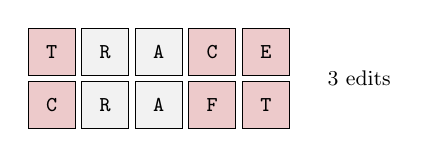
\begin{tikzpicture}[scale=0.85, every node/.style={transform shape}]
    \alignrow{0.8}{T/mRed!30, R/black!5, A/black!5, C/mRed!30, E/mRed!30}{}
    \alignrow{0}{C/mRed!30, R/black!5, A/black!5, F/mRed!30, T/mRed!30}{}
    \node[right] at (4.0,0.4) {\small $3$ edits};
  \end{tikzpicture}
  \end{center}

  \bigskip
  \pause

  \begin{center}
  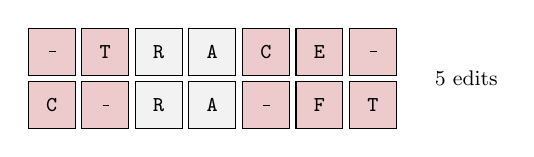
\begin{tikzpicture}[scale=0.85, every node/.style={transform shape}]
    \alignrow{0.8}{\_/mRed!30, T/mRed!30, R/black!5, A/black!5, C/mRed!30, E/mRed!30, \_/mRed!30}{}
    \alignrow{0}{C/mRed!30, \_/mRed!30, R/black!5, A/black!5, \_/mRed!30, F/mRed!30, T/mRed!30}{}
    \node[right] at (5.6,0.4) {\small $5$ edits};
  \end{tikzpicture}
  \end{center}

  \bigskip
  \begin{center}
    The edit distance is the alignment with the \alert{fewest} edits.
  \end{center}
\end{frame}

\begin{frame}{The Table}
  \begin{block}{Definition}
    $ED[i,j]$ = edit distance between $A[1 \ldots i]$ and $B[1 \ldots j]$.
  \end{block}

  \bigskip
  Look at the \alert{last column} of the optimal alignment. There are only
  three possibilities.

  \bigskip
  \begin{center}
  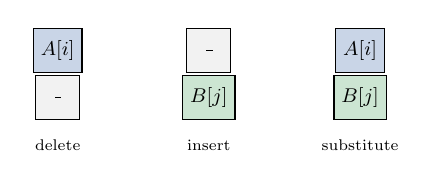
\begin{tikzpicture}[scale=0.8, every node/.style={transform shape},
      bx/.style={draw, minimum size=7mm}]
    % delete
    \node[bx, fill=mLightBlue!30] at (0,0.75) {\small $A[i]$};
    \node[bx, fill=black!5]       at (0,0)    {\small \_};
    \node[below] at (0,-0.55) {\scriptsize delete};
    % insert
    \node[bx, fill=black!5]   at (2.4,0.75) {\small \_};
    \node[bx, fill=mGreen!30] at (2.4,0)    {\small $B[j]$};
    \node[below] at (2.4,-0.55) {\scriptsize insert};
    % substitute
    \node[bx, fill=mLightBlue!30] at (4.8,0.75) {\small $A[i]$};
    \node[bx, fill=mGreen!30]     at (4.8,0)    {\small $B[j]$};
    \node[below] at (4.8,-0.55) {\scriptsize substitute};
  \end{tikzpicture}
  \end{center}
\end{frame}

\begin{frame}{The Three Cases}
  \begin{itemize}
    \item \textbf{Delete $A[i]$:} \; $ED[i-1, j] + 1$.\\
          {\small Transform $A[1 \ldots i-1]$ into $B[1 \ldots j]$, then drop $A[i]$.}
    \pause
    \item \textbf{Insert $B[j]$:} \; $ED[i, j-1] + 1$.\\
          {\small Transform $A[1 \ldots i]$ into $B[1 \ldots j-1]$, then append $B[j]$.}
    \pause
    \item \textbf{Substitute:} \; $ED[i-1, j-1] + \text{diff}(i,j)$, where
          \[
            \text{diff}(i,j) = \begin{cases}
              1 & \text{if } A[i] \ne B[j], \\
              0 & \text{if } A[i] = B[j].
            \end{cases}
          \]
  \end{itemize}
\end{frame}

\begin{frame}{The Recurrence}
  \begin{alertblock}{}
    \[
      ED[i,j] = \min\big\{
        ED[i-1,j] + 1,\;
        ED[i,j-1] + 1,\;
        ED[i-1,j-1] + \text{diff}(i,j)
      \big\}
    \]
  \end{alertblock}

  \bigskip
  Base cases: \; $ED[i, 0] = i$ \; and \; $ED[0, j] = j$. \quad Why?

  \bigskip
  \begin{center}
  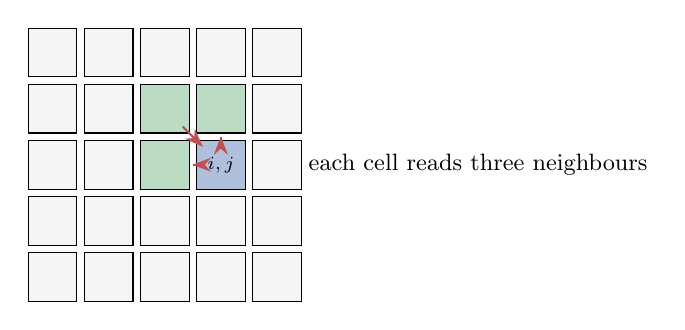
\begin{tikzpicture}[scale=0.95, every node/.style={transform shape},
      c/.style={draw, minimum size=6.5mm}]
    \foreach \i in {0,...,4} \foreach \j in {0,...,4} {
      \node[c, fill=black!4] at (\j*0.75, -\i*0.75) {};
    }
    \node[c, fill=mLightBlue!45] at (0.75*3, -0.75*2) {\scriptsize $i,j$};
    \node[c, fill=mGreen!40]     at (0.75*3, -0.75*1) {};
    \node[c, fill=mGreen!40]     at (0.75*2, -0.75*2) {};
    \node[c, fill=mGreen!40]     at (0.75*2, -0.75*1) {};
    \draw[-{Stealth}, mRed, thick] (0.75*2+0.24, -0.75*1-0.24) -- (0.75*3-0.24, -0.75*2+0.24);
    \draw[-{Stealth}, mRed, thick] (0.75*3, -0.75*1-0.38) -- (0.75*3, -0.75*2+0.38);
    \draw[-{Stealth}, mRed, thick] (0.75*2+0.38, -0.75*2) -- (0.75*3-0.38, -0.75*2);
    \node[right] at (3.3,-1.5) {\small each cell reads three neighbours};
  \end{tikzpicture}
  \end{center}
\end{frame}

\begin{frame}[fragile]{Implementation}
  \begin{lstlisting}[basicstyle=\ttfamily\scriptsize]
function edit_distance(A::String, B::String)
    n, m = length(A), length(B)
    ED = OffsetArray(zeros(Int, n + 1, m + 1), 0:n, 0:m)

    for i in 0:n; ED[i, 0] = i; end      # base cases
    for j in 0:m; ED[0, j] = j; end

    for i in 1:n
        for j in 1:m
            diff = A[i] == B[j] ? 0 : 1
            ED[i, j] = min(
                ED[i - 1, j] + 1,        # delete A[i]
                ED[i, j - 1] + 1,        # insert B[j]
                ED[i - 1, j - 1] + diff  # substitute
            )
        end
    end

    return ED[n, m]
end
  \end{lstlisting}

  \begin{center}
    $O(nm)$ cells, $O(1)$ work each.
  \end{center}
\end{frame}

\begin{frame}{Exercise}
  \begin{center}
    Extend \texttt{edit\_distance} to report the actual edits, not just their
    number.
  \end{center}

  \bigskip
  \begin{center}
    \small Which insertions, deletions, and substitutions turn $A$ into $B$?
  \end{center}
\end{frame}

\begin{frame}{Solution}
  Same idea as $\pi$ in the DAG shortest path: remember \alert{which of the
  three} arguments won.

  \bigskip
  \begin{itemize}
    \item Store a choice table, or recompute the comparison while backtracking.
    \item Start at $(n, m)$ and walk back to $(0,0)$:
      \begin{itemize}
        \item[] from $(i-1,j)$: \; delete $A[i]$
        \item[] from $(i,j-1)$: \; insert $B[j]$
        \item[] from $(i-1,j-1)$: \; substitute, or match if $A[i] = B[j]$
      \end{itemize}
    \item Reverse the list at the end.
  \end{itemize}

  \bigskip
  \begin{center}
    \small The walk visits $O(n + m)$ cells, so this costs nothing extra.
  \end{center}
\end{frame}

\end{document}
